\documentclass[11pt]{report}
\usepackage{geometry}                % See geometry.pdf to learn the layout options. There are lots.
\geometry{a4paper}                   % ... or a4paper or a5paper or ...
% \geometry{landscape}                % Activate for for rotated page geometry
% \usepackage[parfill]{parskip}    % Activate to begin paragraphs with an empty line rather than an indent
\usepackage{lmodern}
\usepackage{graphicx}
\usepackage{amssymb}
\usepackage{epstopdf}
\DeclareGraphicsRule{.tif}{png}{.png}{`convert #1 `dirname #1`/`basename #1 .tif`.png}

\usepackage[colorlinks]{hyperref}
\usepackage{underscore}
\usepackage{textcomp}
\usepackage{xcolor}
\usepackage{parskip}
\usepackage{framed}
\usepackage{listings}
\usepackage{siunitx}
\usepackage[nosolutionfiles]{answers}
\usepackage{tikz}
\usetikzlibrary{arrows,automata,shapes,snakes,patterns,decorations}
\usetikzlibrary{shapes.geometric,shapes.misc}
\usetikzlibrary{shadows}
\usetikzlibrary{calc}
\usetikzlibrary{positioning}
% \usepackage{adjustbox}
\usepackage{todonotes}

\newcommand{\namedtodo}[2][]{%
  % initials of the author (optional) + note in the margin
  {%
    \todo[color={yellow!50},size=\small]{%
      \textbf{TODO [\uppercase{#1}]:}~#2}%
  }}


\lstset{
  language=C,
  basicstyle=\ttfamily\footnotesize,
  commentstyle=\itshape\color{cyan},
  frame=lines
}


\Newassociation{sol}{Solution}{ans}
\newtheorem{ex}{Question}

\newcommand{\normaltilde}{{\raise.17ex\hbox{$\scriptstyle\mathtt{\sim}$}}}
\newcommand{\unixcl}[1]{\texttt{\fcolorbox{black}{gray!20}{\footnotesize#1}}}
\newcommand{\blanc}{\fcolorbox{white}{white}{~}}
\newcommand{\tabkey}{\mbox{$\rightarrow\hspace{-1.4mm}\vert$}}
\title{PRETS/ETERE\\Lab booklet\\2019-2020}
\author{Jean-Luc B\'echennec, Mika\"el Briday, S\'ebastien Faucou}
% \date{}                                           % Activate to display a given date or no date

\hypersetup{linkcolor=red}

\colorlet{shadecolor}{gray!10}

\begin{document}
\maketitle


\chapter{Installation}

\section{Foreword}

It is assumed that you have a basic knowledge of the command line.
If it is not the case, make sure to have the first configuration steps checked
by a member of the teaching team before to proceed with the labs.

\begin{framed}
  Do not copy the commands from the PDF file, the characters you get may not have the correct code and the shell will not understand them.
\end{framed}

When typing shell commands, remember that spaces are important because they separate the command and its arguments. In this document, spaces in commands are represented by a white rectangle like in the following command (it is an example, do not type it):

\noindent
\begin{minipage}{.25\textwidth}
  \unixcl{cd\blanc{}trampoline}
\end{minipage}
\begin{minipage}{.7\textwidth}
  sets the \texttt{trampoline} directory as current directory. This assumes the \texttt{trampoline} directory is a subdirectory of the current one.
\end{minipage}

\section{Setting up the environment}

The tools that we will use have already been installed on the virtual machine:

\begin{itemize}
  \item Trampoline RTOS and the \texttt{goil} configuration generator;

  \item GNU development toolchain including a C compiler and linker (\texttt{gcc}), a debugger (\texttt{gdb}) and an implementation of standard C library (\texttt{glibc}).
\end{itemize}

Trampoline is installed in \unixcl{/opt/trampoline}. \texttt{goil} configuration generator is installed in \unixcl{/usr/local/bin}. All the usefull paths are set in the \unixcl{.profile} startup file of your account.

Now, check that \texttt{goil} is working.
The command \unixcl{goil\blanc{}--version} should print:

\medskip

\begin{shaded*}
  \scriptsize
  \vspace{-1.7mm}
\begin{verbatim}
goil : 3.1.11, build with GALGAS 3.3.12
No warning, no error.
\end{verbatim}
\end{shaded*}

\chapter{The virtual platform}

\section{Overview}

An embedded real-time system interacts with its environment (the plant that it drives) through sensors and actuators.
For this online version of the lab, we will not have access to a real microcontroller-based platform equiped with such devices.
Instead, we are going to use a virtual platform that allows to run TrampolineRTOS application within a Unix process and mimic the behaviour of a very simple environment through a terminal.
This virtual platform is automatically embedded in the program generated by TrampolineRTOS build process when the option \verb|--target| is given to \texttt{goil}.

The virtual platform is equiped with:
\begin{itemize}
  \item
    A set of \textbf{timers} that can be connected to alarms through counters to achieve periodic behaviours or watchdogs.
    The tick of these timers is set to \SI{10}{\milli\second}.
  \item
    Three \textbf{buttons} simulated by keyboard keys:
    \begin{itemize}
      \item
        \texttt{'a'}: The virtual platform raises an interrupt each time it is pressed through Unix signal \verb|SIGTERM|.

      \item
        \texttt{'b'}: The virtual platform raises an interrupt each time it is pressed through Unix signal \verb|SIGTRAP|.

      \item
        \texttt{'q'}: The virtual platform and the TrampolineRTOS application are shut down each time it is pressed.
    \end{itemize}

  \item
    Four \textbf{leds}: \verb|RED|, \verb|GREEN|, \verb|BLUE| and \verb|YELLOW|.
    The state of the leds can be changed through the following functions:
    \begin{itemize}
      \item
        \verb|void set_leds(uint8_t leds)|: switches on the leds given as arguments.
        For instance, to switch on leds \verb|GREEN| and \verb|BLUE|, you can use \verb-set_leds(GREEN | BLUE)-.
      \item
        \verb|void reset_leds(uint8_t leds)|: switches off the leds given as arguments.
        For instance, to switch off leds \verb|RED| and \verb|YELLOW|, you can use \verb-set_leds(RED | YELLOW)-.
    \end{itemize}
    Each time one of these function is called, the state of the leds is printed on the terminal.
  \item
    A \textbf{display}: the control terminal of the process running TrampolineRTOS program and that can be used through functions of the standard C library.
\end{itemize}

\section{Important remarks}

The virtual platform has been packaged in a hurry to create an online version of the labs that can be run during the COVID-19 crisis.
It cannot be considered as a robust and well-tested piece of software.
In order to use it without breaking everything please take into account the following remarks:

\begin{itemize}
  \item
    Although the scheduling of tasks and ISR within the TrampolineRTOS application conforms to OSEK/AUTOSAR OS scheduling policy, remember that this application is embedded in a Unix process that is itself scheduled alongside a bunch of other processes by the underlying non real-time OS.
    Thus, the application are not run in real-tile wrt. physical (wall-clock) time.

  \item
    Moreover, timers of the virtual platform suffer from important jitters due to the fact that (i) the underlying host operating system is not a RTOS, and (ii) Unix signal delivery semantics is piggy-backed on other OS activities and do not trigger preemption by themselves.
    Thus, the application can be notified of the expiry of a timer with a significant tardiness.

  \item
    Do not use input functions from the standard C library as it could interact badly with the virtual buttons.
    Generally speaking, try to avoid using the C standard library that is most of the time not (fully) available on an embedded target.

  \item
    To properly end a line of text to be displayed, you have to use both carriage return and line feed (ie. \verb|\r\n|).
\end{itemize}

% \begin{figure}
%   \begin{center}
%     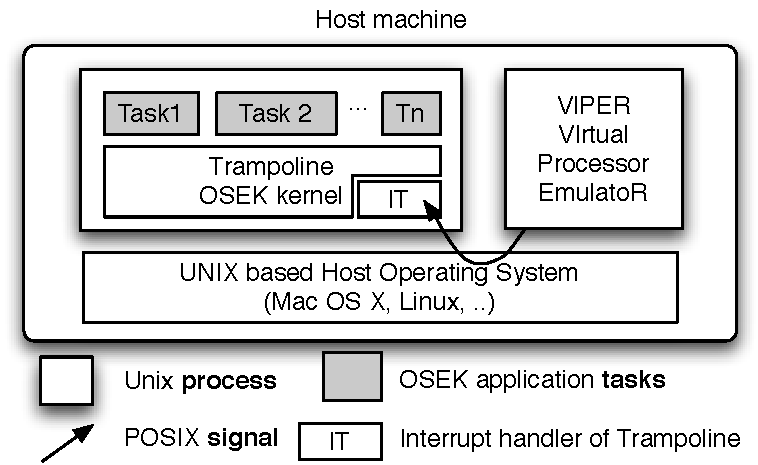
\includegraphics[width=.5\textwidth]{./img/viper.pdf}
%   \end{center}
%   \label{fig:viper}
%   \caption{ViPer}
% \end{figure}

% TODO

\chapter{Lab 1 -- Understanding fixed priority scheduling}

\section{Goal}

The goal of this lab is to become familiar with the development
process of application using Trampoline RTOS, and to understand how fixed priority scheduling works.
We will also see Events.

Trampoline includes an OIL compiler.
It reads a static description of the objects of the application (tasks,
ISRs, events, resources, etc.) and generates the corresponding OS data structures.
In addition to the OIL description, the developer must of course provide the C
source code of the body of tasks and ISRs.


\section{Starting point}

Go into the lab1 directory. There are 2 files:

\begin{description}
  \item[lab1.oil] a minimal OIL description.
  \item[lab1.cpp] a minimal source code.
\end{description}

Edit the lab1.oil file and update the \texttt{TRAMPOLINE\_BASE\_PATH} attribute
in function of your configuration: it should point to the directory where Trampoline is installed.

lab1 is a very simple application with only 1 task named \texttt{task1}. It
starts automatically (\texttt{AUTOSTART = TRUE \{ ... \}} in the OIL file) and
prints "\texttt{Hello world}" on the terminal.

To compile this application, go into the lab1 directory and type (on a single line):

% \namedtodo[JLB]{update path}
\unixcl{\parbox{\linewidth}{%
    goil\blanc{}--target=posix\blanc{}--templates=/opt/trampoline/goil/templates/\blanc{}lab1.oil}}

The \texttt{--target} option is used to define the target system (here we generate the OS level data structures of Trampoline for the \texttt{posix} target).
The \texttt{--templates} option indicates where to find the template files used to generate the configuration of the kernel.

Alongside the C files of the kernel configuration, Goil also generates a build script for the application (files \texttt{make.py} and \texttt{build.py}).

If you change something in the OIL file or in your source code file, you do not need to re-run Goil because the build script should run it when needed.

Continue the build process by typing:

\unixcl{./make.py}

The application and Trampoline OS are compiled and linked together.
The target file is named \texttt{lab1\_exe}.

To run the application, simply run the application:

\unixcl{./lab1_exe}

The program starts and prints the message. As soon as the job of Task1 is terminated, Trampoline gets into idle (starting an internal idle task). To terminate the process, simply type \unixcl{Ctrl+C}.



\section{OS system calls and tasks}

For each question, you should create a copy of the lab1 directory and change its name to \texttt{lab1q1}, \texttt{lab1q2}, \ldots

\subsection{Task activation and scheduling}

The \texttt{ActivateTask()} system call allows to activate a task of the application.

\begin{ex}
  Add two tasks in the system: \texttt{task2} and \texttt{task3}.
  \begin{itemize}
    \item add the declaration of both tasks in the description file (OIL file); \texttt{task2} should have priority 1 and its AUTOSTART attribute should be set to FALSE; \texttt{task3} should have priority 8 and its AUTOSTART attribute should be set to FALSE;
    \item in the implementation file (C file), you should:
      \begin{itemize}
        \item provide the body of each tasks:
          \begin{itemize}
            \item task \texttt{task2} prints "\texttt{==Task2==}" on the terminal;
            \item task \texttt{task3} prints "\texttt{==Task3==}" on the terminal;
          \end{itemize}
        \item and, lastly, modify task \texttt{task1} so that is activates \texttt{task2} and \texttt{task3} (in this order).
      \end{itemize}
  \end{itemize}

  Before to execute the resulting application, draw a schedule and give the text written on the terminal
  Your diagram must clearly show activation, execution and termination of each job using symbols used in the course.
  Then execute the application and check the correctness of your diagram.
\end{ex}

% \subsubsection{Using the debugger to follow the scheduling}
% \namedtodo[SF]{add text on gdb, add \texttt{init.gdb}
% in code.}{TODO}
%
% \begin{ex}
%   Run the application step by step with the debugger and follow the scheduling.
%   Identify precisely the preemption point in the code of each tasks.
% \end{ex}


\subsubsection{Trace evaluation}
% TODO:
% On parle du READY_AND_NEW qui est un état interne… ici, avant?
%
It is not possible to measure timings on this virtual platform. However, The trace allows an analysis of the behavior after execution (post-mortem). To get the trace (after an execution) on standard output:

\begin{lstlisting}
./readTrace.py
\end{lstlisting}

To redirect the output to a file (\texttt{output.txt} here), simply write the command:
\begin{lstlisting}
./readTrace.py >output.txt
\end{lstlisting}


There is one event per line, beginning with the current date (based on \texttt{SystemCounter} value).

Even if the date is the same for several lines, the events (1 per line) are recorded chronologically in the trace file.

Analyze the trace of the current application run, and report on the gantt diagram each events on tasks states.

\subsection{Task chaining}

The \texttt{ChainTask()} system call allows to chain the execution of a task: the calling job terminates and a new job of the target task is created.

\begin{ex}
  % principe base ChainTask
  Starting from the application of question~1, replace the call to \texttt{ActivateTask(task3)} and \texttt{TerminateTask} by a \texttt{ChainTask(task3)} at the end of task \texttt{task1}.
  Draw a schedule of the new system. Then execute the application to check the correctness of your diagram.
  Comment on the differences with the previous application. Explain the differences with the 2 traces.
\end{ex}

\begin{ex}
  % ACTIVATION=1 => 1 fois
  Chain to \texttt{task2} instead of \texttt{task3}.
  Update task \texttt{task2} so that it prints something each time it is executed.
  Draw a schedule of the new system.
  Then execute the application to check the correctness of your diagram.
  Comment on the differences with the previous application.
\end{ex}

\begin{ex}
  % ACTIVATION
  Test the error code returned by ChainTask.
  Modify the OIL file so that ChainTask returns \texttt{E\_OK}.
  Draw a schedule of the new system.
  Then execute the application to check the correctness of your diagram.
  Comment on the differences with the previous application.
\end{ex}

\begin{ex}
  If we wanted to measure the execution time, of \lstinline{ChainTask}, we would have to use a timer as stopwatch. Explain where it should be started and stopped in the following cases:
  \begin{itemize}
    \item fully preemptive scheduling, activation of a higher priority task.
    \item fully preemptive scheduling, activation of a lower priority task.
    \item fully non preemptive scheduling, activation of a higher priority task.
    \item fully non preemptive scheduling, activation of a lower priority task.
  \end{itemize}

  Explain how to use the timer functions for each case and explain the results.
\end{ex}

\section{Extended tasks and synchronization using events}

\textcolor{red}{\emph{For the following exercises, you should use full preemptive scheduling mode.}}

Unlike a basic task, an extended task may wait for an event.
In terms of scheduling, a job is activated when a task is activated or when it leaves the waiting state.

Before to proceed with the following questions, consult the slides of the course to become familiar with events in Trampoline.

% In the OIL file, set the priority of \texttt{task_0} to 8 and add two events \texttt{evt_0} and \texttt{evt_1}. \texttt{evt_0} is used by \texttt{task_0} and \texttt{evt_1} is used by \texttt{task_1}. \texttt{a_task} activates \texttt{task_0} and \texttt{task_1} then sets \texttt{evt_0} and \texttt{evt_1} and terminates. \texttt{task_0} and \texttt{task_1} wait for their event, clear it and terminate.

\begin{ex}
  Based on the application of Question~1, build an application with the following characteristics:
  \begin{itemize}
    \item set priority of \texttt{task2} to 8 (so priorities are 1 for \texttt{task1} and 8 for both \texttt{task2} and \texttt{task3});
    \item add two events, \texttt{evt\_2} and \texttt{evt\_3}:
      \begin{itemize}
        \item \texttt{evt\_2} is set by task \texttt{task1} to task \texttt{task2}.
        \item \texttt{evt\_3} is set by task \texttt{task1} to task \texttt{task3}.
      \end{itemize}
    \item modify the code of the tasks:
      \begin{itemize}
        \item task \texttt{task1} activates \texttt{task2} and \texttt{task3} then sets \texttt{evt\_2} and \texttt{evt\_3} before to terminate.
        \item tasks \texttt{task2} and \texttt{task3} wait for their event, clear it, print their name on stdout (\texttt{==Taskx==}) and terminate.
      \end{itemize}
  \end{itemize}

  Draw a schedule of the new system.
  Then execute the application to check the correctness of your diagram and check that the output order the one awaited. Then, in a second step, explain the trace generated and report each trace event to the schedule of the tasks.

\end{ex}

\begin{ex}
  As in the \lstinline{ChainTask()} service call, give the location where to start and stop a stopwatch to measure the \texttt{SetEvent} service call duration in the following cases:
  \begin{itemize}
    \item fully preemptive scheduling, setting an event to a higher priority tasks that is not waiting for the event.
    \item fully preemptive scheduling, setting an event to a higher priority tasks that is waiting for the event.
    \item fully preemptive scheduling, setting an event to a lower priority tasks that is not waiting for the event.
    \item fully preemptive scheduling, setting an event to a lower priority tasks that is waiting for the event.
  \end{itemize}

\end{ex}

\begin{ex}
  Program an application conforming to the following requirements:

  \begin{itemize}
    \item it is composed of two tasks: \texttt{server} priority 2, \texttt{t1} priority 1.
    \item \texttt{server} is \texttt{AUTOSTART} and built around an infinite loop that activates \texttt{t1} and waits for event \texttt{evt\_1}.
    \item \texttt{t1} prints ``I am t1'' and sets \texttt{evt\_1} of \texttt{server}.
  \end{itemize}

  Before to run the application, draw a schedule of the execution. Add outputs in the bodies of the task to verify your schedule.
\end{ex}

\begin{ex}
  Extend the previous application by adding 2 tasks: \texttt{t2} and \texttt{t3} (priority 1 for both) and 2 events \texttt{evt\_2} and \texttt{evt\_3}. \texttt{server} activates \texttt{t1}, \texttt{t2} and \texttt{t3} and waits for one of the events. When one of the events is set, \texttt{server} activates the corresponding task again.

  Before to run the application, draw a schedule of the execution. Add outputs in the bodies of the task to verify your schedule.
\end{ex}

% ================================================================
\chapter{Lab 2 -- Periodic tasks, Alarms, and ISRs}

\section{Goal}

Real-Time systems are reactive systems which have to trigger processing at certain dates or when the controlled plant reaches a certain state.
You have seen in Lab \#1 how to start processing as a result of an internal event of the system: by activating a task (\texttt{ActivateTask} and \texttt{ChainTask} services) or by setting an event (\texttt{SetEvent} service).
In this lab, you will trigger processing as a result of time elapsing or notification of an external event.
This lab uses the following concepts: counters, alarms, interrupt request, and interrupt service routine.

\section{First application}

You start with a working application composed of an alarm, a task and an isr.

Let us start by analyzing the OIL configuration file.
The alarm \verb-oneSec- is \verb-AUTOSTART-, so it is activated at startup.
Its \verb-CYCLETIME- and \verb-ALARMTIME- are set to \num{100} counter ticks, so it will take its action every \SI{1}{second}.
The action is \verb-ACTIVATETASK- and targets task \verb-task1-, so \verb-task1- will be activated every \SI{1}{second}.
There is also an interrupt service routine (isr for short) named \verb-when_a- that is executed whenever an interrupt request is raised on source \verb-SIGTERM-, ie. when key \verb-a- is pressed in the virtual platform.

Let us now look at the C code.
Whenever isr \verb-when_a- is executed, it toggles the state of LED \verb-GREEN-.
Whenever task \verb-task1- is executed (every \SI{1}{second}), it toggles the state of LED \verb-RED-.

\begin{ex}
  Update the application so that, while still updating the state of LEDs \verb-GREEN- and \verb-RED- as above, it also toggles the state of LED \verb-BLUE- whenever key \verb-b- is pressed in the virtual platform.
\end{ex}

\section{Second application}

The second application will use 2 periodic tasks: \texttt{task1} (priority 2, period \SI{1}{second}) and \texttt{task2} (priority 1, period \SI{1.5}{second}).
At each activation, \texttt{task1} toggles LED \verb-GREEN- while \texttt{task2} toggles LED \verb-RED-.

\begin{ex}
  Draw a schedule of the application between date \num{0} and \SI{12}{seconds} that also shows the state of the LEDs.
  Design, program, and run the application.
\end{ex}


\section{Third application}

In the third application, a \textit{function}\footnote{Here we mean a function of the system, not a function of the C language.} is controlled by external events.
The external event is key \verb-a- has been pressed.
When it occurs, it switches the state of the function from active to inactive and conversely.
When the functions becomes active, it must execute a wake up phase.
To visualize this step, print message \verb-wake up- on the terminal.
Then, the function performs a periodic processing.
To visualize this step, blink a led every \SI{500}{\milli\second}.
Lastly, when it becomes inactive, it must execute a sleeping phase
To visualize this step, print message \verb-sleeping- on the terminal.

Another external event is used to shutdown the system as fast as possible.
This event is key \verb-b- has been pressed.
The shutdown sequence should switch the function to inactive if it is not already in this state before to shutdown the system (using the \texttt{ShutdownOS} service).

\begin{ex}
  Propose a design that uses only basic tasks.
  Draw schedules showing different executions of your design.
  Program, build and test your design.
\end{ex}

\begin{ex}
  Propose a design that uses events and extended tasks.
  Draw schedules showing different executions of your design.
  Program, build and test your design.
\end{ex}

\section{Fourth application}

In this application, you will implement a watchdog.
A watchdog is a mechanism used to take an action after a certain time has elapsed, either to interrupt some on-going processing, or to bound a waiting period.

In your application, each time key \verb-a- is pressed, then key \verb-b- must be pressed within \SI{4}{second}.
In this case, you print the time between the two events.
Otherwise, an error message is displayed.
When key \verb-a- is pressed, subsequent presses on key \verb-a- are ignored for the next \SI{5}{second}.

\begin{ex}
  Specify this behaviour with a state machine.
  What is happening if key \verb-b- is pressed precisely \SI{4}{second} after key \verb-a-?
  Design a solution that handles this situation correctly.
  Draw a schedule of the behaviour of your application in such a scenario (this schedule should show the state of the alarms).
  Program and test your design.
\end{ex}

\section{Fifth application}

In this application, you will program a chase between the LEDs.
In a chase, at any time, only one LED is on and the chase propagates periodically in a given direction.
Your chase will propagate with a period of \SI{500}{\milli\second}, with left to right as its initial direction.

It will be controlled through keys:
\begin{itemize}
  \item
    When key \verb-a- is pressed, it re-initializes the chase.
    If it was not active then it becomes active.
  \item
    When key \verb-b- is pressed, if the chase is active, it is paused.
    If it was paused, then it is resumed but in the opposite direction.
\end{itemize}

\begin{ex}
  Describe the system with a state machine.
  Design a system that implements this state machine.
  Program and test your design.
\end{ex}

%% ================================================================
\chapter{Lab 3 -- Shared object access protection}

To show how to propely access to shared resources, we will use a bad program that allows to corrupt a shared global variable which is not protected against concurrent writes. This has been presented in the course. This lab will show different ways to prevent this wrong behavior by using resources (standard and internal) or other solutions (preemption and priority).

To ensure that the compiler does not hide our bug, update the value of the \texttt{CFLAGS} key in the OIL file: replace option \texttt{-Os} by \texttt{-O0} to turn off all optimizations.

\section{Application requirements}
\label{sec:sharedrez}

%\label{{shared_res_app}

The diagram of figure~\ref{fig:appdiag} describes the application.
It is composed of 3 tasks that share 2 global variables,\texttt{val} and \texttt{activationCount}, {\bf declared with the volatile keyword}.
The tasks in the system are:
\begin{itemize}
  \item A background task called \texttt{bgTask}, activated at startup. In an infinite loop it increments then decrements the global variable \texttt{val}. This task has priority 1.
  \item A periodic task called \texttt{periodicTask} that activates a job every 50ms. This periodic task increments the global variable \texttt{activationCount}. If \texttt{activationCount} is odd, \texttt{val} is incremented, otherwise it is decremented. This task has priority 10.
  \item A periodic task \texttt{displayTask} that runs every 2 second and prints \texttt{val}. This task has priority 2.
\end{itemize}

\def\alarm#1#2{
  \node[alarm](#1) [#2] {};
  \coordinate (a) at ($(#1.north)$);
  \coordinate (b) at ($(#1.north east)$);
  \coordinate (c) at ($(#1.north west)$);
  \coordinate (d) at ($(#1)$);
  \draw[thick] ($(a)+(-0.1,0)$) rectangle ($(a)+(0.1,0.1)$);
  \draw[rotate=-45,thick] ($(b)+(-0.05,0)$) rectangle ($(b)+(0.05,0.1)$);
  \draw[rotate=45,thick] ($(c)+(-0.05,0)$) rectangle ($(c)+(0.05,0.1)$);
  \draw ($(d)+(0.3,0)$) -- (d) -- ($(d)+(0,0.3)$);
  \node [font=\scriptsize,below=0.5mm of #1] {{\em Alarm}}
}

\def\sharedvar#1#2#3{
  \node (#1) [#2] {#1};
  \coordinate (a) at ($(#1.north #3) + (0,0.2)$);
  \coordinate (b) at ($(#1.south #3) + (0,-0.2)$);
  \draw[ultra thick] (a) -- (b);
  \draw ($(a)+(-0.1,0)$) -- ($(a)+(0.1,0)$);
  \draw ($(b)+(-0.1,0)$) -- ($(b)+(0.1,0)$)
}

\def\varrect#1{
  \draw ($(#1.south west)$) rectangle ($(#1.north east)$)
}

\begin{figure}[htbp] %  figure placement: here, top, bottom, or page
  \centering
  \begin{tikzpicture}[
    task/.style={draw,very thick,fill=white,drop shadow={opacity=0.25},text width=2.5cm, text centered, minimum height=1.5cm},
    alarm/.style={draw,thick,circle,fill=white,drop shadow={opacity=0.25},text width=.5cm}
    ]
    \node[task](periodicTask) at (0,0) {periodicTask};
    \node[task](bgTask) [above=of periodicTask] {bgTask};
    \node[task](displayTask) [above=of bgTask] {displayTask};
    \alarm{activateDisplay}{left=20mm of displayTask};
    \alarm{activatePeriodic}{left=20mm of periodicTask};
    \sharedvar{val}{left=of bgTask}{east};
    % \sharedvar{activationCount}{right=of periodicTask}{west};
    \sharedvar{stdout}{right=of displayTask}{west};
    \varrect{stdout};
    \draw [thick,<->] (val.east) -- (bgTask.west);
    \draw [thick,->] (val.north east) -- ++(5mm,0) |- ($(displayTask.south west) + (0,2mm)$);
    \draw [thick,<->] (val.south east) -- ++(5mm,0) |- ($(periodicTask.north west) + (0,-2mm)$);

    \draw [thick,->] (activateDisplay.east) -- ++(5mm,0) -- ++(0,1.5mm) -- ++(3mm,-3mm) -- ++ (0mm,1.5mm) -- (displayTask);
    \node at ($(activateDisplay.east) + (6.5mm,-3mm)$) {2s};
    \node[font=\scriptsize] at ($(activateDisplay.east) + (9mm,3mm)$) {{\em ActivateTask}};
    \draw [thick,->] (activatePeriodic.east) -- ++(5mm,0) -- ++(0,1.5mm) -- ++(3mm,-3mm) -- ++ (0mm,1.5mm) -- (periodicTask);
    \node at ($(activatePeriodic.east) + (6.5mm,-3mm)$) {50ms};
    \node[font=\scriptsize] at ($(activatePeriodic.east) + (9mm,3mm)$) {{\em ActivateTask}};
    % \draw [thick,<->] (activationCount.west) -- (periodicTask);
    % \draw [thick,->] (activationCount.north west) -- ++(-5mm,0) |- ($(displayTask.south east) + (0,2mm)$);
    \draw [thick,->] (displayTask) -- (stdout);
  \end{tikzpicture}
  \caption{Application diagram}
  \label{fig:appdiag}
\end{figure}

\begin{ex}
  Before programming the application, gives the expected sequence of values for val.
  Design, program, and run the application.
  Now, decrease gradually the period of task \texttt{periodicTask} and observe the sequence of values of val.
  Comment.
\end{ex}


% Compile again your application but add a \unixcl{CFLAGS = "-O3"} in the OIL file. This flag
% makes the C compiler optimize the assembly code.

% \begin{ex}
%   Is it the same behavior as in previous question? Why?
% \end{ex}



\section{Global variable protection}

% Remove the \unixcl{CFLAGS = "-O3"} from the OIL file. As shown in the course, we must protect the access to the global variable.

Update the OIL file and the C program to protect the access to the global variable \texttt{val}. Use a resource to do it.

The resource priority is automatically computed by goil according to the priorities of the tasks which use it.

The OIL compiler generates many files in the directory bearing the same name as the oil file (without the .oil suffix). Among them 3 are of interest for this lab:
\begin{itemize}
  \item \texttt{tpl_app_define.h}
  \item \texttt{tpl_app_config.h}
  \item \texttt{tpl_app_config.c}
\end{itemize}

The file \texttt{tpl_app_config.c} contains the task descriptors among other data structures. These structures are commented.

\begin{ex} ~
  \begin{itemize}
    \item
      Recall the computation rule of the ceiling priority of a resource with the immediate ceiling protocol.
      According to this rule, what should be the ceiling priority of the resource?
    \item
      Find the actual ceiling priority in \texttt{tpl_app_config.c}. Is it the expected value? If not, is it a problem?
  \end{itemize}
\end{ex}

% To observe the impact of the priority ceiling protocol, use the following function to observe the priority of the jobs during their execution.

% \begin{lstlisting}[language=C]
% void displayIdAndCurrentPriority()
% {
%   TaskType id;
%   GetTaskID(&id);
%   if (id >= 0)
%   {
%     tpl_priority prio = (tpl_dyn_proc_table[id]->priority) >> PRIORITY_SHIFT;
%     lcd.print("Id=");
%     lcd.print(id);
%     lcd.print(", Prio=");
%     lcd.print(prio);
%   }
% }
% \end{lstlisting}

% And you have to add the following line at start of your C file:

% \begin{lstlisting}[language=C]
% #include "tpl_os_task_kernel.h"
% \end{lstlisting}


\section{Protection with an internal resource}

An internal resource is automatically taken when the job gets the CPU, and released when it terminates. Replace the standard resource by an internal resource in the OIL file. Remove the \texttt{GetResource} and \texttt{ReleaseResource} in the C file.

\begin{ex}~
  \begin{itemize}
    \item
      What happens? Why?
    \item
      How to solve the problem? Draw a schedule of a correct implementation of the system. Program this solution.
  \end{itemize}
\end{ex}


\section{Protection using a single priority level}

\begin{ex}
  Modify the OIL file: remove the resource and set the priorities so that all tasks share the same priority. Draw a schedule of the system.
\end{ex}

\section{Protection using fully non preemptive scheduling mode}

\begin{ex}
  Modify the OIL file: all tasks are now non preemptive. Draw a schedule of the system.
\end{ex}

%%%% TODO : mettre à jour la question qui suit. Maintenant que Trampoline est installé dans /opt
%%%% et que les fonctions du TFT et de l'expandeur sont en libs dans machines/, les
%%%% étudiants ne peuvent plus ajouter les ressources dans le code.

% \section{Upgrading the coro\_utils function}
%
% \begin{ex}
%   As explained in section~\ref{sec:coroutils}, both the screen and the IO
%   expander use the SPI interface of the MCU. Thus, to ensure coherency of SPI
%   transactions, we have avoided using both devices in the same application.
%   However, using resources, it is possible to enforce mutual exclusions
%   between concurrent tasks that use the SPI.
%   Design and program such an application.
% \end{ex}

\chapter{Lab4\\Internal communication}

\section{Basic usage}

Internal communication allows task to exchange data under the control of the RTOS.
It can be used in the place of communication through shared global variables.
It is usually preferable to use internal communication rather than shared global variables because (i) it tends to improve application design by making data flows explicits, and (ii) it limits the bugs resulting by a wrong use of synchronization tools.

In the starting application for this lab, task \verb|send| sends a message to task \verb|receive|.
The former is activated at system startup, while the latter is activated when a message is delivered.
Build, run, and study the code of this application to gain basic knowledge of internal communication.
More details are provided in the course and in the reference documents available on TrampolineRTOS github page (bottom of homepage).

\begin{ex}
  Design an application with two periodic tasks (period \SI{1}{second} and \SI{1.5}{seconds}). At every activation, each task sends a message containing its number of activation since system startup.
  A third task is activated whenever one of this messages arrives and prints the identity of the sender and its number of activation.
  The receiver task shall process only one message per activation.
  It shall not miss any message.

  Explain your design and draw a schedule. Program and test your design.
\end{ex}

\section{Many-to-many communication pattern}

OSEK messaging supports \emph{many-to-many} communication.
This is done by having more than one receiving messages connected to the same sending message.

\begin{ex}
  Design an application with a periodic task that sends random data with values in $[0,100]$.
  Two other tasks are receiving this flow:
  \begin{itemize}
    \item
      The first one is activated whenever a new message is available and print its value;
    \item
      The second one is an extended task that is notified of the arrival of a new value by an event.
      When the event is received, it prints the average value over the last 10 messages (or less if less than 10 messages have been received so far).
  \end{itemize}

  Explain your design and draw a schedule. Program and test your design.
\end{ex}

\section{Filtering}

OSEK messaging also supports filtering.
Filters are predicate attached to sending or receiving message objects, used to decide if data should be sent or received.

\begin{ex}
  Add the following filters to your application:
  \begin{itemize}
    \item
      The task activated upon message arrival is now acticated only if the value is below \num{20} or above \num{80}.
      In the former case it prints message \verb-low val- and in the latter one it prints \verb-high val-.
    \item
      The other task is notified only one every two messages.
      Notice that it should nonetheless process all messages.
  \end{itemize}
\end{ex}

\section{Application design}

\begin{ex}
  Propose a new design for the application described in section~\ref{sec:sharedrez} that uses messages instead of shared variables.

  Explain your design and draw a schedule. Program and test your design.
\end{ex}

\end{document}
